\chapter{Função potência e polinomial}


\section{Paridade de uma função}

 \begin{obs}
  Dada um função $f: \R \rightarrow \R$.

\begin{itemize}
    \item   Dizemos que $f$ é uma \textbf{função par} se, para todo $x \in \R$,
\begin{equation*}
f(-x)= f(x) \ .
\end{equation*}
  \item Dizemos que $f$ é uma \textbf{função ímpar} se, para todo $x \in \R$,
\begin{equation*}
f(-x)= - f(x) \ .
\end{equation*}
\end{itemize}
\end{obs}


 \begin{exem}
  \begin{enumerate}[a)]
   \item A função $f(x)= x$ é uma função ímpar;
\begin{equation*}
f(-x)= -x= -f(x) 
\end{equation*}
   \item A função $f(x)= x^2$ é uma função par;
\begin{equation*}
f(-x)= (-x)^2= x^2 = f(x) 
\end{equation*}
   \item A função $f(x)= x^3$ é uma função ímpar.
\begin{equation*}
f(-x)= (-x)^3= -x^3= -f(x)
\end{equation*}

\item Note que uma função pode não ser par nem ímpar. A função $f(x)=x+1$ não é par nem ímpar pois para $x=1$ temos que $f(1)=2$ e $f(-1)=0$.
  \end{enumerate}
 \end{exem}

 \begin{exem}
  Vamos analisar a paridade de função modular $f(x)= \abs{x}$.
    Veja que $f(-x)=\abs{-x}=\abs{x}=f(x)$. Portanto $f$ é uma função par.
 \end{exem}

 \section{Função potência}

\begin{obs}
Uma \textbf{função potência} é uma função real $f:A\to\R$ da forma
\begin{equation*}
    f(x)=x^n,
\end{equation*}
onde $n$ é um valor constante.
\end{obs}

Devemos analisar a função de acordo com a escolha do valor de $n$.

\subsection{Caso $n$ natural ímpar}

Vejamos os gráficos para os casos $n=1, 3$ e $5$:
\begin{center}
  \begin{tikzpicture}[scale=0.7]
    \tkzInit[xmin=-3, xmax=3, xstep=1, ymin=-3,ymax=3]
        %\tkzDrawXY
        \tkzAxeXY
        %\tkzGrid
        %\tkzLabelX[text=blue,below = 3pt,]
        
        \tkzFct[thick,red]{x}
        \tkzText[below right, black](2,2){$y=x$}
        %\tkzFct[thick,red]{x**3}
        %\tkzFct[thick,red,domain=-1.5:1.5]{x**5}

        %\tkzDefPoint(1.5,0.25){A}
        %\tkzDefPointByFct[ref=A, with=a](-1)
        %\tkzDefPoint(0,2){A}
        %\tkzDefPoint(0.5,2.25){B}
        %\tkzPointShowCoord[xlabel=$\frac{3}{2}$]((1.5,0.25))
        %\tkzDrawPoint[fill=red, size=3](A)
        %\tkzDrawPoint[fill=red, size=3](B)
        
    \end{tikzpicture}
      \begin{tikzpicture}[scale=0.7]
    \tkzInit[xmin=-3, xmax=3, xstep=1, ymin=-3,ymax=3]
        %\tkzDrawXY
        \tkzAxeXY
        
        %\tkzFct[thick,red]{x}
        \tkzFct[thick,red]{x**3}
        \tkzText[below right, black](2,2){$y=x^3$}
        %\tkzFct[thick,red,domain=-1.5:1.5]{x**5}

        %\tkzDefPoint(1.5,0.25){A}
        %\tkzDefPointByFct[ref=A, with=a](-1)
        %\tkzDefPoint(0,2){A}
        %\tkzDefPoint(0.5,2.25){B}
        %\tkzPointShowCoord[xlabel=$\frac{3}{2}$]((1.5,0.25))
        %\tkzDrawPoint[fill=red, size=3](A)
        %\tkzDrawPoint[fill=red, size=3](B)
        
    \end{tikzpicture}
    \begin{tikzpicture}[scale=0.7]
    \tkzInit[xmin=-3, xmax=3, xstep=1, ymin=-3,ymax=3]
        %\tkzDrawXY
        \tkzAxeXY
        
        %\tkzFct[thick,red]{x}
        %\tkzFct[thick,red]{x**3}
        \tkzText[below right, black](2,2){$y=x^5$}
        \tkzFct[thick,red,domain=-1.5:1.5]{x**5}

        %\tkzDefPoint(1.5,0.25){A}
        %\tkzDefPointByFct[ref=A, with=a](-1)
        %\tkzDefPoint(0,2){A}
        %\tkzDefPoint(0.5,2.25){B}
        %\tkzPointShowCoord[xlabel=$\frac{3}{2}$]((1.5,0.25))
        %\tkzDrawPoint[fill=red, size=3](A)
        %\tkzDrawPoint[fill=red, size=3](B)
        
    \end{tikzpicture}
\end{center}

    Podemos notar que:
    \begin{itemize}
        \item Todos os gráficos passam pela origem;
        \item Todos os gráficos passam pelos pontos $(1,1)$ e $(-1,-1)$;
        \item São funções ímpares;
        \item A imagem delas é o conjunto dos reais $\R$.
    \end{itemize}

\subsection{Caso $n$ natural par}

Vejamos os gráficos para os casos $n=2, 4$ e $6$:
\begin{center}
  \begin{tikzpicture}[scale=0.7]
    \tkzInit[xmin=-3, xmax=3, xstep=1, ymin=-1,ymax=4]
        %\tkzDrawXY
        \tkzAxeXY
        %\tkzLabelX[text=blue,below = 3pt,]
        
        \tkzFct[thick,red]{x**2}
        \tkzText[below right, black](2,2){$y=x^2$}
        %\tkzFct[thick,red]{x**3}
        %\tkzFct[thick,red,domain=-1.5:1.5]{x**5}

        %\tkzDefPoint(1.5,0.25){A}
        %\tkzDefPointByFct[ref=A, with=a](-1)
        %\tkzDefPoint(0,2){A}
        %\tkzDefPoint(0.5,2.25){B}
        %\tkzPointShowCoord[xlabel=$\frac{3}{2}$]((1.5,0.25))
        %\tkzDrawPoint[fill=red, size=3](A)
        %\tkzDrawPoint[fill=red, size=3](B)
        
    \end{tikzpicture}
      \begin{tikzpicture}[scale=0.7]
    \tkzInit[xmin=-3, xmax=3, xstep=1, ymin=-1,ymax=4]
        %\tkzDrawXY
        \tkzAxeXY
        
        %\tkzFct[thick,red]{x}
        \tkzFct[thick,red,domain=-1.5:1.5]{x**4}
        \tkzText[below right, black](2,2){$y=x^4$}
        %\tkzFct[thick,red,domain=-1.5:1.5]{x**5}

        %\tkzDefPoint(1.5,0.25){A}
        %\tkzDefPointByFct[ref=A, with=a](-1)
        %\tkzDefPoint(0,2){A}
        %\tkzDefPoint(0.5,2.25){B}
        %\tkzPointShowCoord[xlabel=$\frac{3}{2}$]((1.5,0.25))
        %\tkzDrawPoint[fill=red, size=3](A)
        %\tkzDrawPoint[fill=red, size=3](B)
        
    \end{tikzpicture}
    \begin{tikzpicture}[scale=0.7]
    \tkzInit[xmin=-3, xmax=3, xstep=1, ymin=-1,ymax=4]
        %\tkzDrawXY
        \tkzAxeXY
        
        %\tkzFct[thick,red]{x}
        %\tkzFct[thick,red]{x**3}
        \tkzText[below right, black](2,2){$y=x^6$}
        \tkzFct[thick,red,domain=-1.5:1.5]{x**6}

        %\tkzDefPoint(1.5,0.25){A}
        %\tkzDefPointByFct[ref=A, with=a](-1)
        %\tkzDefPoint(0,2){A}
        %\tkzDefPoint(0.5,2.25){B}
        %\tkzPointShowCoord[xlabel=$\frac{3}{2}$]((1.5,0.25))
        %\tkzDrawPoint[fill=red, size=3](A)
        %\tkzDrawPoint[fill=red, size=3](B)
        
    \end{tikzpicture}
\end{center}

    Podemos notar que:
    \begin{itemize}
        \item Todos os gráficos passam pela origem;
        \item Todos os gráficos passam pelos pontos $(1,1)$ e $(-1,1)$;
        \item São funções pares;
        \item A imagem delas é o conjunto $\R_{+}=[0,\infty)$.
    \end{itemize}

    \subsection{Caso $n$ negativo ímpar}

Vejamos o gráfico para o caso $f(x)=x^{-1}=\frac{1}{x}$:
\begin{center}
  \begin{tikzpicture}[scale=0.7]
    \tkzInit[xmin=-3, xmax=3, xstep=1, ymin=-3,ymax=3]
        %\tkzDrawXY
        \tkzAxeXY
        %\tkzLabelX[text=blue,below = 3pt,]
        
        \tkzFct[thick,red,domain=0.1:3]{x**(-1)}
        \tkzFct[thick,red,domain=-3:-0.1]{x**(-1)}
        \tkzText[below right, black](2,2){$y=\frac{1}{x}$}
        %\tkzFct[thick,red]{x**3}
        %\tkzFct[thick,red,domain=-1.5:1.5]{x**5}

        %\tkzDefPoint(1.5,0.25){A}
        %\tkzDefPointByFct[ref=A, with=a](-1)
        %\tkzDefPoint(0,2){A}
        %\tkzDefPoint(0.5,2.25){B}
        %\tkzPointShowCoord[xlabel=$\frac{3}{2}$]((1.5,0.25))
        %\tkzDrawPoint[fill=red, size=3](A)
        %\tkzDrawPoint[fill=red, size=3](B)
        
    \end{tikzpicture}
\end{center}

    Podemos notar que:
    \begin{itemize}
        \item O maior domínio é $\R^{*}$;
        \item A imagem é $\R^{*}$;
        \item O gráfico passa pelos pontos $(1,1)$ e $(-1,-1)$;
        \item É uma função ímpar;
        \item Quando $x$ aumenta muito, as imagens se aproximam de zero. Se $x$ aumenta muito em valor absoluto, porém com sinal negativo, as imagens também se aproximam de zero;
        \item Quando $x$ se aproxima de zero por valores positivos, as imagens são cada vez maiores. Quando $x$ se aproxima de zero por valores negativos, as imagens são também cada vez menores.
    \end{itemize}

Pode-se verificar que as demais funções desse tipo, por exemplo, $f(x)=x^{-3}=\frac{1}{x^3}$ ou $f(x)=x^{-5}=\frac{1}{x^5}$ possuem um padrão gráfico semelhante ao da função $\frac{1}{x}$.

    

        \subsection{Caso $n$ negativo par}

Vejamos o gráfico para o caso $f(x)=x^{-2}=\frac{1}{x^2}$:
\begin{center}
  \begin{tikzpicture}[scale=0.7]
    \tkzInit[xmin=-3, xmax=3, xstep=1, ymin=-1,ymax=4]
        %\tkzDrawXY
        \tkzAxeXY
        %\tkzLabelX[text=blue,below = 3pt,]
        
        \tkzFct[thick,red,domain=0.1:3]{x**(-2)}
        \tkzFct[thick,red,domain=-3:-0.1]{x**(-2)}
        \tkzText[below right, black](2,2){$y=\frac{1}{x^2}$}
        %\tkzFct[thick,red]{x**3}
        %\tkzFct[thick,red,domain=-1.5:1.5]{x**5}

        %\tkzDefPoint(1.5,0.25){A}
        %\tkzDefPointByFct[ref=A, with=a](-1)
        %\tkzDefPoint(0,2){A}
        %\tkzDefPoint(0.5,2.25){B}
        %\tkzPointShowCoord[xlabel=$\frac{3}{2}$]((1.5,0.25))
        %\tkzDrawPoint[fill=red, size=3](A)
        %\tkzDrawPoint[fill=red, size=3](B)
        
    \end{tikzpicture}
\end{center}

    Podemos notar que:
    \begin{itemize}
        \item O maior domínio é $\R^{*}$;
        \item A imagem é $(0,\infty)$;
        \item O gráfico passa pelos pontos $(1,1)$ e $(-1,1)$;
        \item É uma função par;
        \item Quando $x$ aumenta muito, as imagens se aproximam de zero. Se $x$ aumenta muito em valor absoluto, porém com sinal negativo, as imagens também se aproximam de zero;
        \item Quando $x$ se aproxima de zero por valores positivos ou negativos, as imagens são cada vez maiores.
    \end{itemize}
    
    Pode-se verificar que as demais funções desse tipo, por exemplo, $f(x)=x^{-4}=\frac{1}{x^4}$ ou $f(x)=x^{-6}=\frac{1}{x^6}$ possuem um padrão gráfico semelhante ao da função $\frac{1}{x^2}$.


    \subsection{Caso $n$ seja da forma $\frac{1}{k}$}

    A função $f(x)=x^{1/k}=\sqrt[k]{x}$.

    Para $n=\frac{1}{2}$, esta é a função raiz quadrada $f(x)=\sqrt{x}$. O gráfico desta função é:
\begin{center}
  \begin{tikzpicture}[scale=0.7]
    \tkzInit[xmin=-1, xmax=6, xstep=1, ymin=-1,ymax=4]
        %\tkzDrawXY
        \tkzAxeXY
        %\tkzLabelX[text=blue,below = 3pt,]
        
        \tkzFct[thick,red,domain=0:6]{sqrt(x)}
        \tkzText[below right, black](2,1.5){$y=\sqrt{x}$}
        %\tkzFct[thick,red]{x**3}
        %\tkzFct[thick,red,domain=-1.5:1.5]{x**5}

        %\tkzDefPoint(1.5,0.25){A}
        %\tkzDefPointByFct[ref=A, with=a](-1)
        %\tkzDefPoint(0,2){A}
        %\tkzDefPoint(0.5,2.25){B}
        %\tkzPointShowCoord[xlabel=$\frac{3}{2}$]((1.5,0.25))
        %\tkzDrawPoint[fill=red, size=3](A)
        %\tkzDrawPoint[fill=red, size=3](B)
        
    \end{tikzpicture}
\end{center}

    Podemos notar que:
    \begin{itemize}
        \item O maior domínio é $\R_{+}$;
        \item A imagem é $\R_{+}$;
        \item O gráfico passa pelos pontos $(0,0)$ e $(1,1)$;
        \item O gráfico é a parte superior da parábola descrita pela equação $x=y^2$.
    \end{itemize}

Para $n=\frac{1}{3}$, esta é a função raiz cúbica $f(x)=\sqrt[3]{x}$. O gráfico desta função é:
\begin{center}
  \begin{tikzpicture}[scale=0.7]
    \tkzInit[xmin=-4, xmax=4, xstep=1, ymin=-3,ymax=3]
        %\tkzDrawXY
        \tkzAxeXY
        %\tkzLabelX[text=blue,below = 3pt,]
        
        \tkzFct[thick,red,domain=0:4]{x**(0.33)}
        \tkzFct[thick,red,domain=-4:0]{-abs(x)**(0.33)}
        \tkzText[below right, black](2,1.5){$y=\sqrt[3]{x}$}
        %\tkzFct[thick,red]{x**3}
        %\tkzFct[thick,red,domain=-1.5:1.5]{x**5}

        %\tkzDefPoint(1.5,0.25){A}
        %\tkzDefPointByFct[ref=A, with=a](-1)
        %\tkzDefPoint(0,2){A}
        %\tkzDefPoint(0.5,2.25){B}
        %\tkzPointShowCoord[xlabel=$\frac{3}{2}$]((1.5,0.25))
        %\tkzDrawPoint[fill=red, size=3](A)
        %\tkzDrawPoint[fill=red, size=3](B)
        
    \end{tikzpicture}
\end{center}

    Podemos notar que:
    \begin{itemize}
        \item O maior domínio é $\R$;
        \item A imagem é $\R$;
        \item O gráfico passa pelos pontos $(0,0)$, $(1,1)$ e $(-1,-1)$;
        \item O gráfico corresponde à cúbica descrita pela equação $x=y^3$.
    \end{itemize}
    
%  \textbf{Função raiz quadrada}

%  É a função $f: \R_{+} \to \R_{+}$ dada por $f(x)= \sqrt{x}$, cujo gráfico é:

%   \begin{figure}[H]
% \centering
%    \fbox{\includegraphics[width=6cm]{./cap_funcao/figs/funcaoraizquadrada}}
%    \caption{Função raiz quadrada}
%  \end{figure}

%  Note que neste caso o domínio da função são apenas os números reais positivos, já que não existe raiz quadrada de número negativo.

%  \textbf{Função raiz cúbica}

%  É a função $f: \R \to \R$ dada por $f(x)= \sqrt[3]{x}$, cujo gráfico é:

%   \begin{figure}[H]
% \centering
%    \fbox{\includegraphics[width=6cm]{./cap_funcao/figs/funcaoraizcubica}}
%    \caption{Função raiz cúbica}
%  \end{figure}

%  \textbf{Função recíproca}

%  É a função $f: \R \setminus \{0\} \to \R$ dada por $f(x)= \frac{1}{x}$, cujo gráfico é:

%   \begin{figure}[H]
% \centering
%    \fbox{\includegraphics[width=6cm]{./cap_funcao/figs/funcaoreciproca}}
%    \caption{Função recíproca}
%  \end{figure}

%  Neste caso o domínio da função é o conjunto $\R \setminus \{0\}$, pois não existe divisão por $0$ (zero).

\section{Funções polinomiais de grau \texorpdfstring{$n$}{n}}

\begin{obs}
As funções $f: \R \to \R$ com a seguinte regra geral:
\begin{equation*}
f(x) = a_0 + a_1 x + a_2 x^2 + a_3 x^3 + \cdots + a_n x^n
\end{equation*}
para $\{a_0, a_1, a_2, a_3, \ldots a_n\} \in \R$ e $n \in \N$, tais que $a_n \neq 0$ são denominadas \\ \textbf{funções polinomiais de grau $n$}.
\end{obs}

Observe que as funções de 1ª e 2ª grau são exemplos de funções polinomiais. Vejamos agora um breve estudo sobre as funções polinomiais de 3º grau.

\subsection{Funções do 3º grau}
As funções do 3º grau ou funções cúbicas são funções $f: \R \rightarrow \R$ dadas por:
\begin{equation*}
f(x)= ax^3 + bx^2 + cx + d \ ,
\end{equation*}
para certos $a, b, c, d \in \R$ com $a \neq 0$. As \textbf{raízes} ou \textbf{zeros} das funções de 3º grau são os $x \in \R$ tais que $ax^3 + bx^2 + cx + d=0$. Assim as funções de 3º grau podem classificadas de acordo com suas raízes em 4 casos:
\begin{itemize}
 \item 3 raízes reais distintas. Por exemplo, o gráfico da função $f(x)= x^3-x^2-2x=x(x-2)(x+1)$ é:
 \begin{center}
    \begin{tikzpicture}[scale=1]
    \tkzInit[xmin=-4, xmax=4, xstep=1, ymin=-3,ymax=3]
        %\tkzDrawXY
        \tkzAxeXY
        %\tkzLabelX[text=blue,below = 3pt,]
        
        \tkzFct[thick,red]{x*(x-1)*(x+2)}
        %\tkzText[below right, black](2,1.5){$y=\sqrt[3]{x}$}
        %\tkzFct[thick,red]{x**3}
        %\tkzFct[thick,red,domain=-1.5:1.5]{x**5}

        %\tkzDefPoint(1.5,0.25){A}
        %\tkzDefPointByFct[ref=A, with=a](-1)
        %\tkzDefPoint(0,2){A}
        %\tkzDefPoint(0.5,2.25){B}
        %\tkzPointShowCoord[xlabel=$\frac{3}{2}$]((1.5,0.25))
        %\tkzDrawPoint[fill=red, size=3](A)
        %\tkzDrawPoint[fill=red, size=3](B)
        
    \end{tikzpicture}
\end{center}
 \item 3 raízes reais sendo duas delas iguais. Por exemplo, o gráfico da função $f(x)= 2x^3-3x^2+1=2(x+\frac{1}{2})(x-1)^2$ é:
 \begin{center}
    \begin{tikzpicture}[scale=1]
    \tkzInit[xmin=-4, xmax=4, xstep=1, ymin=-3,ymax=3]
        %\tkzDrawXY
        \tkzAxeXY
        %\tkzLabelX[text=blue,below = 3pt,]
        
        \tkzFct[thick,red]{2*x**3-3*x**2+1}
        %\tkzText[below right, black](2,1.5){$y=\sqrt[3]{x}$}
        %\tkzFct[thick,red]{x**3}
        %\tkzFct[thick,red,domain=-1.5:1.5]{x**5}

        %\tkzDefPoint(1.5,0.25){A}
        %\tkzDefPointByFct[ref=A, with=a](-1)
        %\tkzDefPoint(0,2){A}
        %\tkzDefPoint(0.5,2.25){B}
        %\tkzPointShowCoord[xlabel=$\frac{3}{2}$]((1.5,0.25))
        %\tkzDrawPoint[fill=red, size=3](A)
        %\tkzDrawPoint[fill=red, size=3](B)
        
    \end{tikzpicture}
\end{center}
 \item 3 raízes reais iguais. Por exemplo, o gráfico da função $f(x)= -x^3+6x^2-12x+8=-(x-2)^3$ é:
 \begin{center}
    \begin{tikzpicture}[scale=1]
    \tkzInit[xmin=-4, xmax=4, xstep=1, ymin=-3,ymax=3]
        %\tkzDrawXY
        \tkzAxeXY
        %\tkzLabelX[text=blue,below = 3pt,]
        
        \tkzFct[thick,red]{-(x-2)**3}
        %\tkzText[below right, black](2,1.5){$y=\sqrt[3]{x}$}
        %\tkzFct[thick,red]{x**3}
        %\tkzFct[thick,red,domain=-1.5:1.5]{x**5}

        %\tkzDefPoint(1.5,0.25){A}
        %\tkzDefPointByFct[ref=A, with=a](-1)
        %\tkzDefPoint(0,2){A}
        %\tkzDefPoint(0.5,2.25){B}
        %\tkzPointShowCoord[xlabel=$\frac{3}{2}$]((1.5,0.25))
        %\tkzDrawPoint[fill=red, size=3](A)
        %\tkzDrawPoint[fill=red, size=3](B)
        
    \end{tikzpicture}
\end{center}
 \item 1 raiz real (e duas raízes complexas). Por exemplo, o gráfico da função $f(x)= 2x^3-3x^2+2$ é:
 \begin{center}
    \begin{tikzpicture}[scale=1]
    \tkzInit[xmin=-4, xmax=4, xstep=1, ymin=-3,ymax=3]
        %\tkzDrawXY
        \tkzAxeXY
        %\tkzLabelX[text=blue,below = 3pt,]
        
        \tkzFct[thick,red]{2*x**3-3*x**2+2}
        %\tkzText[below right, black](2,1.5){$y=\sqrt[3]{x}$}
        %\tkzFct[thick,red]{x**3}
        %\tkzFct[thick,red,domain=-1.5:1.5]{x**5}

        %\tkzDefPoint(1.5,0.25){A}
        %\tkzDefPointByFct[ref=A, with=a](-1)
        %\tkzDefPoint(0,2){A}
        %\tkzDefPoint(0.5,2.25){B}
        %\tkzPointShowCoord[xlabel=$\frac{3}{2}$]((1.5,0.25))
        %\tkzDrawPoint[fill=red, size=3](A)
        %\tkzDrawPoint[fill=red, size=3](B)
        
    \end{tikzpicture}
\end{center}
\end{itemize}

% Estes casos estão representados nos gráficos abaixo, onde consideramos sempre $a> 0$, o caso $a< 0$ é análogo.




%   \begin{figure}[H]
%   \fbox{\subfigure[$a < 0$]{\includegraphics[width=7cm,height=5cm]{./cap_funcao/figs/g1}}}
%   \fbox{\subfigure[$a < 0$]{\includegraphics[width=7cm,height=5cm]{./cap_funcao/figs/g2}}}
%   \end{figure}

%  \begin{figure}[H]
%   \fbox{\subfigure[$a < 0$]{\includegraphics[width=7cm,height=5cm]{./cap_funcao/figs/g3}}}
%   \fbox{\subfigure[$a < 0$]{\includegraphics[width=7cm,height=5cm]{./cap_funcao/figs/g4}}}
%   \caption{Gráficos de funções do 3º grau}
%  \end{figure}


  

%   \textbf{Função floor}

%   É a função $f: \R \to \R$ dada por $f(x)= \lfloor {x} \rfloor$, cujo gráfico é:

%    \begin{figure}[H]
%  \centering
%     \fbox{\includegraphics[width=6cm]{./cap_funcao/figs/funcaofloor}}
%     \caption{Função floor}
%   \end{figure}

%   Esta função aplicada em um número $x$ tem como imagem a parte inteira do número $x$.

%   \textbf{Função ceil}

%   É a função $f: \R \to \R$ dada por $f(x)= \lceil {x} \rceil$, cujo gráfico é:

%    \begin{figure}[H]
%  \centering
%     \fbox{\includegraphics[width=6cm]{./cap_funcao/figs/funcaoceil}}
%     \caption{Função ceil}
%   \end{figure}

%   Esta função aplicada em um número $x$ tem como imagem o menor inteiro maior ou igual a $x$.

\begin{secExercicios}

    \begin{exer}
        Esboce os gráficos das funções a seguir, determinando seu domínio, imagem e verificando se é função par ou ímpar:
        \begin{enumerate}[a)]
            \item $f(x)=-x^3$
            \item $f(x)=x^4$
            \item $f(x)=x^{-3}$
            \item $f(x)=x^{\frac{1}{5}}$
            \item $f(x)=\sqrt[4]{x}$
            \item $f(x)=x^{-4}$
        \end{enumerate}
    \end{exer}

    \begin{exer}
        Determine se a função é par, ímpar ou nenhum dos dois:
        \begin{enumerate}[a)]
            \item $f(x)=x^5+x$
            \item $f(x)=1-x^4$
            \item $f(x)=2x-x^2$
        \end{enumerate}
    \end{exer}

    \begin{exer}
        Determine o(s) ponto(s) de interseção entre os gráficos das funções $f(x)=x$ e $g(x)=\frac{1}{x}$.
    \end{exer}
    
    \begin{exer}
        Determine a equação da reta que passa pelos pontos de interseção dos gráficos das funções $f(x)=\frac{1}{x}$ e $g(x)=\sqrt[3]{x}$.
    \end{exer}

    \begin{exer}
        Encontre a expressão para uma função cúbica $f$ tal que $f(1)=6$ e $f(-1)=f(0)=f(2)=0$.
    \end{exer}

    \begin{exer}
        (UNICAMP-2020) Seja a função polinomial do terceiro grau $f(x) = x^3 - x^2 - 2x + 1$, definida para todo número real $x$. A figura abaixo exibe o gráfico de $y=f(x)$, no plano cartesiano, em que os pontos $A$, $B$ e $C$ têm a mesma ordenada. Determine a distância entre os pontos $A$ e $C$.
         \begin{center}
    \begin{tikzpicture}[scale=0.7]
    \tkzInit[xmin=-4, xmax=4, xstep=1, ymin=-3,ymax=3]
        \tkzDrawXY[noticks]
        %\tkzAxeXY
        %\tkzLabelX[text=blue,below = 3pt,]
        
        \tkzFct[thick]{x**3 - x**2 - 2*x + 1}
        %\tkzText[below right, black](2,1.5){$y=\sqrt[3]{x}$}
        %\tkzFct[thick,red]{x**3}
        %\tkzFct[thick,red,domain=-1.5:1.5]{x**5}

        %\tkzDefPoint(1.5,0.25){A}
        %\tkzDefPointByFct[ref=A, with=a](-1)
        %\tkzDefPoint(0,2){A}
        \tkzDefPoint[label= right:$A$](-1,1){A}
        \tkzDefPoint[label= right:$B$](0,1){B}
        \tkzDefPoint[label= right:$C$](2,1){C}
        %\tkzDrawSegment(A,B)
        %\tkzDrawSegment[line width=1pt](A,C)
        \tkzPointShowCoord[noxdraw](A)
        \tkzPointShowCoord[noxdraw](C)
        \tkzDrawPoint[fill=black, size=3](A)
        \tkzDrawPoint[fill=black, size=3](B)
        \tkzDrawPoint[fill=black, size=3](C)
        
        
    \end{tikzpicture}
\end{center}
    \end{exer}
    
\end{secExercicios}